% !TeX spellcheck = it_IT
% !TeX root = ../../compl.tex
\section{Problemi $\NP$-completi}

Un problema di decisione $X$ è \NPc se $x \in \NP$ e per qualunque $Y \in \NP$ vale $Y \polred X$. Intuitivamente, i problemi di decisione $\NP$-completi sono i "più difficili" in $\NP$, infatti vale il seguente.\\

\begin{fact}
    Sia $X$ un qualunque problema \NPc. Allora $X \in \P$ se e solo $P \equiv \NP$.
\end{fact}
\begin{proof}
    Se $\P \equiv \NP$ allora $X \in \P$. D'altra parte, se $X$ è \NPc, allora dato un qualunque $Y \in \NP$ vale $Y \polred X$. Per ipotesi, $X$ è risolvibile in tempo polinomiale, di conseguenza lo è $Y$, quindi $Y \in \P$, da cui otteniamo $\NP \subseteq \P$. Abbiamo già dimostrato come $\P \subseteq \NP$, quindi $\P \equiv \NP$.
\end{proof}

Non è chiaro che esistano problemi \NPc. Potrebbero esserci due problemi $X', X'' \in \NP$ tali che non esiste nessun altro $X \in \NP$ tale che $X' \polred X$ e $X'' \polred X$. Oppure, potrebbe esserci una sequenza infinita di problemi in $\NP$ del tipo $X_1 \polred X_2 \polred \dots$ tale che non esista un problema più difficile degli altri.

Un \textbf{circuito} è un grafo diretto aciclico (senza loop, archi multipli e pesi) avente un unico nodo senza archi uscenti chiamato nodo di output.  I nodi senza archi entranti possono avere un valore di verità preassegnato. I nodi senza archi entranti e senza valori preassegnati sono chiamati nodi di input. I nodi rimanenti hanno uno o due archi entranti e sono etichettati da un operatore booleano $\wedge$, $\vee$, $\neg$ in modo tale che nodi $\wedge$ e $\vee$ abbiano esattamente due archi entranti e nodi $\neg$ abbiamo esattamente un arco entrante.

Un circuito calcola una funzione booleana $f: \left\{0,1\right\}^n \rightarrow \left\{0,1\right\}$ dove $n$ è il numero dei nodi di input. Dato un assegnamento $\left(b_1, \dots, b_n\right) \in \left\{0,1\right\}^n$ di valori di verità ai nodi di input, calcoliamo $f\left(b_1, \dots, b_n\right)$ come il valore di verità del nodo di output ottenuto valutando in cascata i valori di verità di ciascun nodo. La valutazione di un nodo avviene applicando l'operatore logico che lo etichetta ai valori di verità dei nodi all'altro capo degli archi entranti. Se la valutazione di ogni nodo avviene in tempo costante, allora l'intero circuito viene valutato in tempo lineare nel numero dei nodi.

Sostanzialmente, si tratta del parsing tree di una funzione booleana.

Il problema di decisione \textbf{Circuit Satisfiability} (CS) ha istanze che rappresentano circuiti. La funzione di decisione $q$ è tale che $q(I) = 1$ se e solo se esiste un assegnamento ai nodi di input del circuito $I$ tale che il nodo di output assume valore 1. In altre parole, $q(I) = 1$ se e solo se la funzione $f$ calcolata dal circuito è tale che $f\left(b_1, \dots, b_n\right) = 1$ per un qualche $\left(b_1, \dots, b_n\right) \in \left\{0,1\right\}^n$. \\

\begin{theorem}[Cook-Levin]
    CS è \NPc.
\end{theorem}
\begin{proof}
    La dimostrazione completa è omessa in quanto lunga e tecnicamente complessa. Si basa sul fatto che ogni algoritmo con un tempo di esecuzione polinomiale nella lunghezza dell'input può essere implementato da una famiglia di circuiti $C_1, C_2, \dots$ dove $C_n$ ha $n$ nodi di input e un numero polinomiale di altri nodi. Per simulare l'algoritmo su un input $I$ di lunghezza $n$, calcoliamo l'output del circuito $C_n$ con input $I$.

    Per dimostrare che un problema $X \in \NP$ è polinomialmente riducibile a CS consideriamo un certificatore polinomiale $B$ per $X$, il quale esiste in quanto $X \in \NP$. Costruiamo la famiglia di circuiti $C_1', C_2', \dots$ tale che $C_n'$ ha $n + p(n)$ nodi senza archi entranti e un numero polinomiale in $n$ di altri nodi, dove $p(\cdot)$ è il polinomio che limita la lunghezza dei certificati di $B$. Per ogni $n$, $C_n'$ simula $B$ su istanze $I$ di lunghezza $n$. Data un'istanza $I \in \I$ di lunghezza $n$, sia $C_n' (I, \cdot)$ il circuito $C_n'$ dove i valori dei primi $n$ nodi senza archi entranti sono preassegnati ai bit di $I$, mentre i rimanenti $p(n)$ nodi sono di input. Allora $C_n'(I, \cdot)$ simula il certificatore polinomiale $B(I, \cdot)$. Ovvero, $C_n'(I, \cdot)$ è soddisfacibile se e solo se esiste $z \in \left\{0,1\right\}^\ast$ con $|z| \leq p(|I|)$ tale che $B(I, z) = 1$.
\end{proof}

Dimostriamo ora un caso particolare del teorema di Cook-Levin, ovvero che un particolare problema di decisione è polinomialmente riducibile a CS. Il problema è 2-IS, con istanze $I$ che rappresentano grafi semplici, mentre la funzione di decisione $q$ è tale che $q(I) = 1$ se e solo se il grafo $I$ contiene un insieme indipendente di tagli almeno 2. \\

\begin{theorem}
    2-IS $\polred$ CS.
\end{theorem}
\begin{proof}
    Sia $G = (V,E)$ un grafo su $n$ vertici. Gli archi del grafo $G$ possono essere codificati con una stringa $I_G \in \left\{0,1\right\}^N$ dove $N = \binom{n}{2}$, ogni bit rappresenta una coppia di vertici e un arco fra una coppia di vertici è codificato ponendo a 1 il bit corrispondente. Indichiamo con $B$ il certificatore polinomiale per 2-IS, il quale esiste in quanto 2-IS $\in \NP$.

    Dimostriamo ora come costruire in tempo polinomiale nella descrizione di $G$ un circuito $C$ con $\binom{n}{2} + n$ nodi senza archi entranti tale che $C (I_G, \cdot)$ è soddisfacibile se e solo se esiste una stringa $z$ di lunghezza $n$ tale che $B(I_G, z) = 1$. Questo completa la riduzione, in quanto per calcolare la funzione di decisione di $2-IS$ su un'istanza $I_G$ è sufficiente costruire $C$, invocare l'oracolo per CS e produrre in output la risposta dell'oracolo.

    Notiamo che i certificati per 2-IS possono essere codificati con una stringa $z \in \left\{0,1\right\}^n$ che ha almeno due occorrenze di 1 nelle posizioni corrispondenti ai vertici che formano un insieme indipendente nel grafo.

    Costruiamo quindi un circuito con $\binom{n}{2} +n$ nodi di input tale che i primi $\binom{n}{2}$ vengono utilizzati per codificare $I_G$ e i successivi $n$ nodi vengono utilizzati per codificare un certificato $z$. A questo punto, usiamo $2 \binom{n}{2} - 1$ per verificare che $z$ contenga almeno due occorrenze di 1 e usiamo $2\binom{n}{2}$ nodi interni per verificare che non ci sia un arco fra i nodi scelti dal certificato.
\end{proof}


\begin{figure}[t]
    \centering
    \begin{minipage}{0.24\linewidth}
        \resizebox{\linewidth}{!}{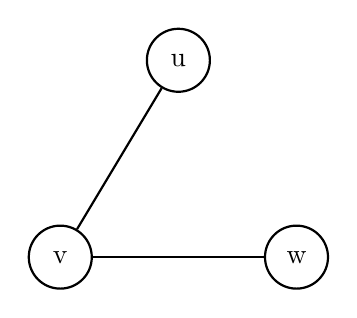
\begin{tikzpicture}[
    vertex/.style={
        circle,
        draw=black,
        thick,
        minimum size=8mm,
        inner sep=0pt
    }
    ]
    \node[vertex] (v) at (0,0) {v};
    \node[vertex] (w) at (3,0) {w};
    \node[vertex] (u) at (1.5, 2.5) {u};

    \draw[thick] (v) -- (u);
    \draw[thick] (v) -- (w);
\end{tikzpicture}}
    \end{minipage}
    \hfill
    \begin{minipage}{0.74\linewidth}
        \resizebox{\linewidth}{!}{\begin{forest}
    % Tree configuration
    for tree={
        circle,
        draw,
        l sep=20pt,
        s sep=15pt,
        edge={Stealth-}
    }
    [$\wedge$, label={[align=center] right: IS di dimensione \\ almeno 2?}
    [$\neg$, label={left: IS?}
    [$\vee$, label={[align=center]left: Entrambi i lati di un \\ arco sono stai scelti?}
    [$\vee$, tier=m2
    [$\wedge$, tier=mid, name=v1
    [u-v, tier=bot, name=d1]
    ]
    [$\wedge$, tier=mid, name=v2
    [u-w, tier=bot, name=d2]
    ]
    ]
    [$\wedge$, tier=mid, name=v3
    [v-w, tier=bot, name=d3]
    ]
    ]
    ]
    [$\vee$, tier=m2, label={[align=center] right: Set di almeno \\ 2 elementi?}
    [$\vee$
    [$\wedge$, tier=b2, name=c1
    [u, tier=bot, name=b1]
    ]
    [$\wedge$, tier=b2, name=c2
    [v, tier=bot, edge={draw=none}, name=b2]
    ]
    ]
    [$\wedge$, tier=b2, name=c3
    [w, tier=bot, name=b3]
    ]
    ]
    ]
    % Draw the arrow using TikZ syntax relative to the forest nodes
    \draw[Stealth-] (v1) to (c1);
    \draw[Stealth-] (v2) to (c2);
    \draw[Stealth-] (v3) to (c3);
    \draw[Stealth-] (c1) to (b2);
    \draw[Stealth-] (c2) to (b1);
    \draw[Stealth-] (c2) to (b3);
    \draw[Stealth-] (c3) to (b2);
    \node[fit=(d1)(d3), label={[align=center]below:$\binom{n}{2}$ input fissi per gli archi \\ (descrizione del grafo)}] {};
    \node[fit=(b1)(b3), label={[align=center]below:$n$ input \\ (nodi nell'IS)}] {};
\end{forest}}
    \end{minipage}
    \caption{Riduzione da 2-IS a CS}
    \label{fig:IStree}
\end{figure}

In Figura \ref{fig:IStree} si può vedere un esempio:
\begin{itemize}
    \item Al di sopra dei nodi di input per $z$, ogni nodo $\wedge$ chiede "sono stati scelti questi due nodi?"; la restante parte destra dell'albero controlla solamente che siano stati scelti almeno due nodi

    \item Il risultato della "scelta" viene messo in $\wedge$ con la codifica degli archi presenti

    \item I risultati vengono messi in $\vee$, quindi risulta 1 se e solo se sono stati scelti due nodi che hanno un arco presente tra loro; viene invertito per avere 1 nel caso di Independent Set

    \item La radice si occupa di controllare che l'input rappresenti un Independent set (sottoalbero di sinistra) di dimensione almeno 2 (sottoalbero di destra)
\end{itemize}

Una volta che abbiamo stabilito che un certo problema è \NPc, possiamo trovarne molti altri usando la seguente osservazione. \\

\begin{fact}
    Se $Y$ è \NPc e $X \in \NP$ è tale che $Y \polred X$, allora anche $X$ è \NPc.
\end{fact}
\begin{proof}
    Sia $Z \in \NP$ qualunque. Allora $Z \polred Y$. Ma dato che $Y \polred X$, allora $Z \polred X$, il che implica che $X$ è \NPc.
\end{proof}

Possiamo subito applicare questa osservazione dimostrando quanto segue. \\

%TODO: cercare dim? Maybe
\begin{theorem}
    CS $\polred$ 3-SAT.
\end{theorem}
\begin{proof}
    Omessa.
\end{proof}

Dato che CS è \NPc, ne segue che anche 3-SAT è \NPc. Ricordando inoltre che 3-SAT $\polred$ Independent Set $\polred$ Vertex Cover $\polred$ Set Cover, ne deduciamo che tutti questi problemi sono \NPc. Al contrario di 3-SAT che è \NPc, 2-SAT (ovvero usando clausole da esattamente due letterali) è un problema risolvibile in tempo lineare.

Si noti che ogni formula booleana può essere equivalentemente rappresentata come un circuito (ovvero un'istanza di CS) o come una formula CNF (ovvero un'istanza di SAT) in modo che tali istanze abbiano lunghezza polinomiale nella lunghezza della formula. Inoltre, ogni istanza $I$ di SAT può essere rappresentata come un'istanza di 3-SAT di lunghezza polinomiale in $|I|$ (queste dimostrazioni sono il processo per la dimostrazione omessa precedentemente).

Al contrario, non è sempre possibile rappresentare una formula booleana in DNF in modo che la DNF abbia lunghezza polinomiale nella lunghezza della formula. Se questo fosse possibile avremmo che $\P \equiv \NP$. La soddisfacibilità di una DNF è decidibile in tempo lineare controllando che esista almeno una congiunzione della formula che è soddisfacibile da un qualche assegnamento.

Si noti che la definizione di $\NP$ è asimmetrica: dato un problema $X = (\I, q) \in \NP$, se $q(I) = 1$ allora esiste un certificato polinomiale $z$ tale che $B(I, z) = 1$ dove $B$ denota il certificatore polinomiale per $X$. Se invece $q(I) = 0$ allora la definizione ci garantisce solo che $B(I,z) = 0$ per un numero esponenziale di certificati $z$. Questa asimmetria si riscontra quanto consideriamo problemi $\bar X = (\I, \bar q)$ che sono complementari di problemi $X = (\I, q)$. Per \textit{complementare} di $X$ si intende che $\bar q(I) = 0$, ma non sappiamo se esista un certificato polinomiale che certifichi $\bar q (I) = 1$. Per esempio, se $X$ è Independent Set, allora per certificare $\bar q(I) = 1$ dovremmo trovare un certificato polinomiale che attesti che il grafo \textbf{non} contenga un insieme indipendente di taglia $k$.

Quindi non è chiaro se $\NP \equiv \coNP$, dove $\coNP$ indica la classe dei problemi di decisione complementari di problemi in $\NP$ (se $\NP$ è l'insieme dei problemi di cui posso verificare una soluzione/certificato in tempo polinomiale, per i problemi in $\coNP$ non è possibile avere una soluzione verificabilemente corretta in tempo polinomiale, è invece possibile verificare in tempo polinomiale che una soluzione restituisce 0).

Lo scenario è differente per $\P$: $X \in \P$ se e solo se $\bar X \in \P$. Infatti $X = (\I, q) \in \P$ implica che esiste un algoritmo per calcolare $q$ in tempo polinomiale. Ma allora si può anche calcolare $\bar q$ in tempo polinomiale semplicemente calcolando $q$ e complementando l'output. Quindi $\P \equiv \coP$.

Dimostrare che $\coNP \not \equiv \NP$ sarebbe un progresso ancora maggiore che dimostrare $\P \not \equiv \NP$. Vale infatti la seguente cosa. \\

\begin{fact}
    Se $\coNP \not \equiv \NP$ allora $\P \not \equiv \NP$.
\end{fact}
\begin{proof}
    Dimostriamo la contrapositiva, ovvero che $\P \equiv \NP$ implica $\coNP \equiv \NP$. Intuitivamente, dato che $\P$ è chiuso rispetto all'operazione di complemento, se $\P \equiv \NP$ allora deve essere che $\coNP \equiv \NP$. Formalmente
    $$ X \in \NP \Longleftrightarrow X \in \P \Longleftrightarrow \bar X \in \P \Longleftrightarrow \bar X \in \NP \Longleftrightarrow X \in \coNP $$
    Il che conclude la dimostrazione.
\end{proof}

Possiamo caratterizzare i problemi $X = (\I, q) \in \coNP$ tramite l'esistenza di un polinomio $p(\cdot)$ e di un certificatore polinomiale $B$, calcolabile in tempo polinomiale, tale che $q(I) = 0$ se e solo se esiste una stringa $z \in \left\{0,1\right\}^{p(|I|)}$ tale che $B(I,z) = 0$. Si noti che $\P \subseteq \coNP$, infatti, potendo implementare $q$ in tempo polinomiale, si può calcolare $B(I,z)$ ignorando $z$ e restituendo $q(I)$.

Una classe particolarmente interessante è quella dei problemi in $\NP \cap \coNP$. Sia $X = (\I, q)$ un tale problema
\begin{itemize}
    \item Dato che $X \in \NP$ esiste un polinomio $p(\cdot)$ e un certificatore polinomiale $B$ tale che $q(I) = 1$ se e solo se esiste una stringa $z \in \left\{0,1\right\}^{p(|I|)}$ tale che $B(I,z) = 1$

    \item Dato che $X \in \coNP$ esiste un polinomio $p'(\cdot)$ e un certificatore polinomiale $B'$ tale che $q(I) = 0$ se e solo se esiste una stringa $z' \in \left\{0,1\right\}^{p'(|I|)}$ tale che $B'(I, z') = 0$
\end{itemize}

Quindi i problemi in $\NP \cap \coNP$ sono tali che per ogni istanza $I$ esiste un certificato polinomiale, sia quando $q(I) = 1$ sia quando $q(I) = 0$.

Si noti che se $X \in \P$ allora $X \in \NP$ ed anche $X \in \coNP$. Quindi $\P \subseteq \NP \cap \coNP$. D'altra parte non si sa se $\P \not \equiv \NP \cap \coNP$. Ovvero non si sa se esistono problemi le cui istanze hanno sempre certificati brevi ma tuttavia non sono risolubili in tempo polinomiale.

% End of np.pdf